\chapter{Data Analysis II}

\section{Beam Particle Identification}
Figures of beam contaminants in our beam PID line. 
Table of beam purity reference to Jon's thesis paper

\section{Edge Cuts}
As seen in Fig.~\ref{fig:edge}, edges of the measurement volume of the TPC we can see several edge effects distortion the clusters positions. The last pads on the edges of the pad-plane naturally have no neighbors on the outsides, therefore their cluster position is biased towards the inside of the TPC. Also since we measure a finite window in time for the vertical direction, pulses near the edge of the time-bucket window are clipped and the reconstructed times are biased towards inside the TPC volume. 

The number of affected clusters is small, but the deviation at the end of the track is enough to start causing issues in the momentum reconstruction. Simple cuts around the left,right, top, and bottom of the TPC remove these clusters from the analysis,

\begin{equation*}
  |x|\geq420~\mathrm{mm},\quad y\leq-522+\mathrm{y_o}~\mathrm{mm},
  \quad\mathrm{and}\quad y\geq-64+\mathrm{(Hit\ Shift)}~\mathrm{mm}.
\label{eq:hitshift}
\end{equation*}

\begin{figure}[!htb]
    \centering
    \begin{subfigure}[t]{0.45\textwidth}
        \centering
        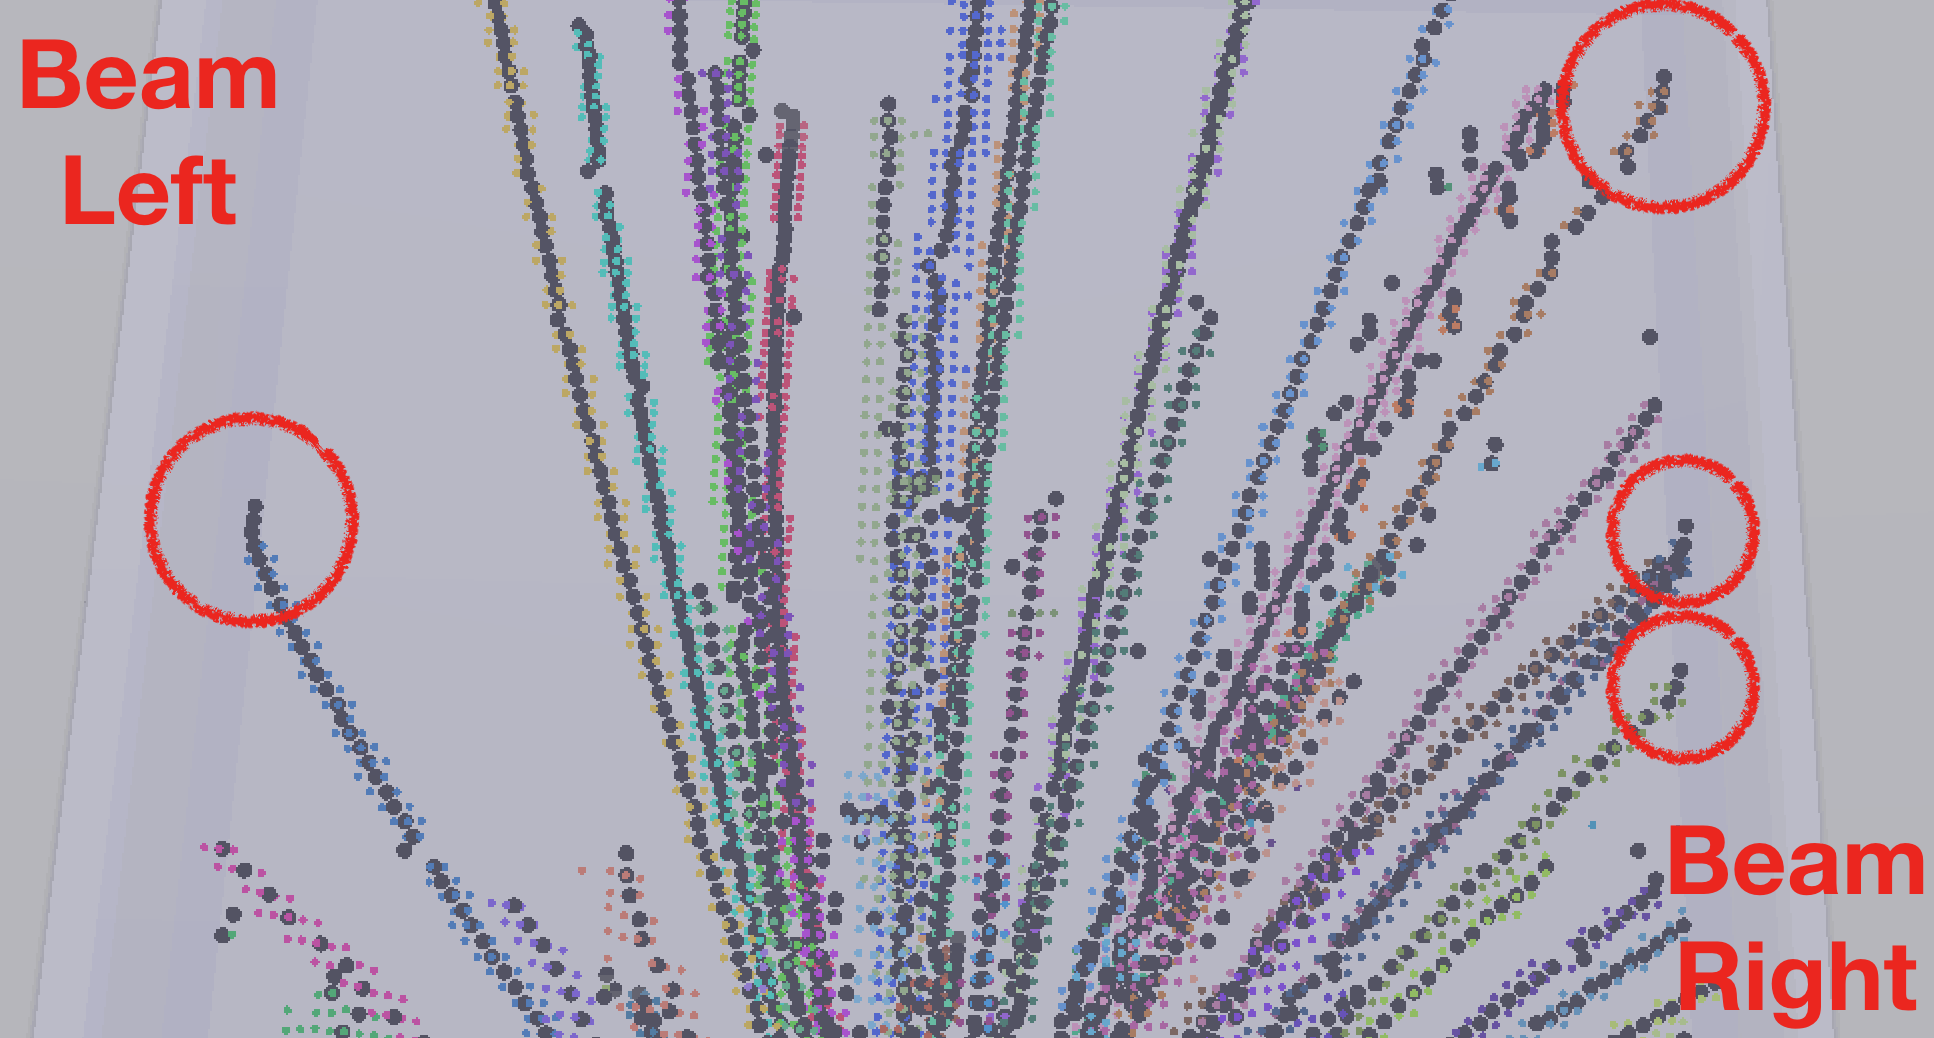
\includegraphics[width=\linewidth]{clusterLR.png} 
        \caption{Generic} \label{fig:mom_S_before}
    \end{subfigure}
    \hfill
    \begin{subfigure}[t]{0.45\textwidth}
        \centering
        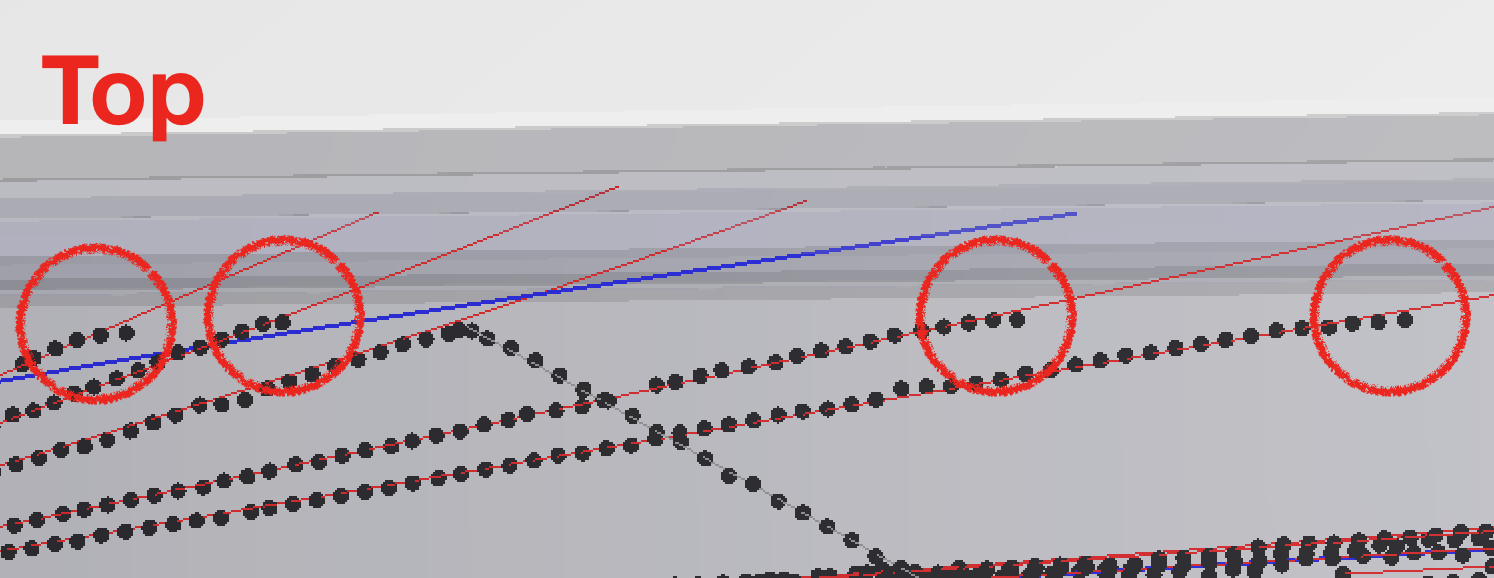
\includegraphics[width=\linewidth]{clusterTop.png} 
        \caption{Competitors} \label{fig:mom_L_before}
    \end{subfigure}
    
    \begin{subfigure}[t]{0.45\textwidth}
        \centering
        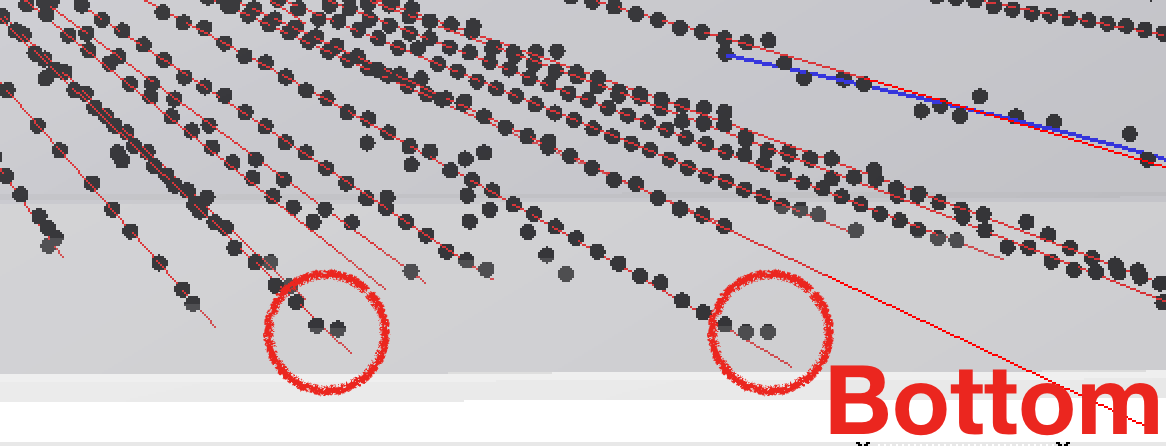
\includegraphics[width=\linewidth]{clusterBottom.png} 
        \caption{Generic} \label{fig:mom_S_after}
    \end{subfigure}
   
\label{fig:edge}
\end{figure}

\section{High Density Cut}
The density of tracks near the target region is very high and most of electronics information from this region is inaccurate in both timing and charge value. Hits lying within an semi-ellipsoidal cut region around the target are removed from the software and not included in the track and momentum reconstruction. 

Add picture of ellipsoid 

\section{Beam angle selection}
The beam is bent by the magnetic field before hitting the target. The BDCs track the beam outside of the magnet. The beam is then propagated through the magnetic field until the target position. The beam angle on target is categorized by two angles $\theta_{a_{proj}}$ and $\theta$

\begin{figure}[!htb]
    \centering
    \begin{subfigure}[t]{0.45\textwidth}
        \centering
        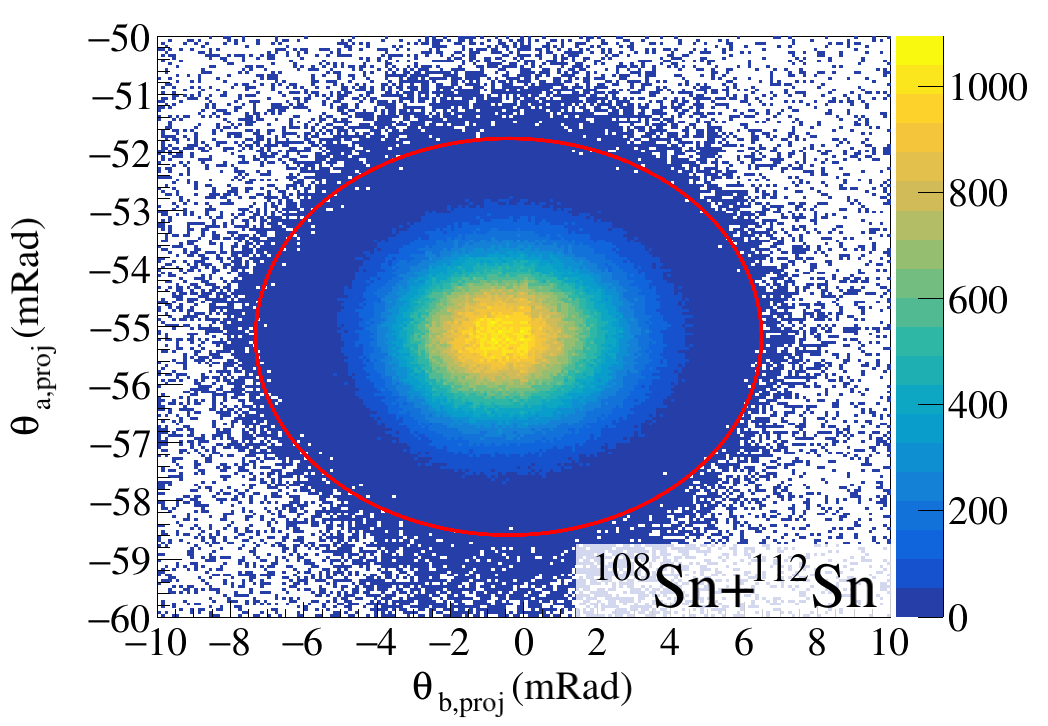
\includegraphics[width=\linewidth]{beamAngle-Sn108.png} 
        \caption{Generic} \label{fig:mom_S_before}
    \end{subfigure}
    \hfill
    \begin{subfigure}[t]{0.45\textwidth}
        \centering
        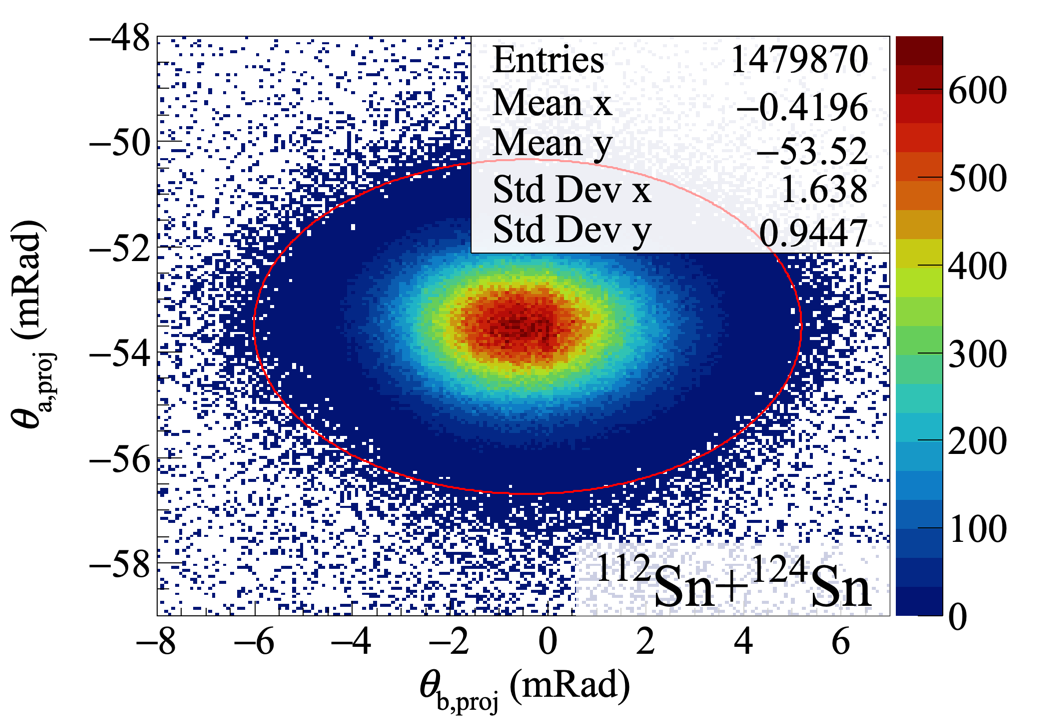
\includegraphics[width=\linewidth]{beamAngle-Sn112.png} 
        \caption{Competitors} \label{fig:mom_L_before}
    \end{subfigure}
    
    \begin{subfigure}[t]{0.45\textwidth}
        \centering
        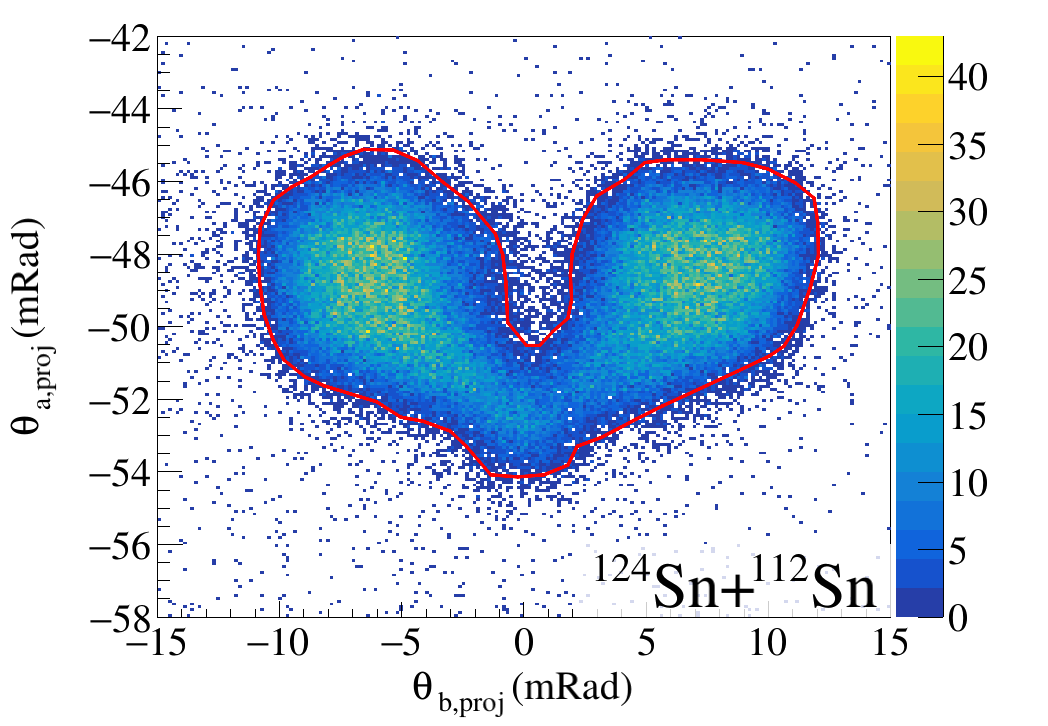
\includegraphics[width=\linewidth]{beamAngle-Sn124.png} 
        \caption{Generic} \label{fig:mom_S_after}
    \end{subfigure}
    \hfill
    \begin{subfigure}[t]{0.45\textwidth}
        \centering
        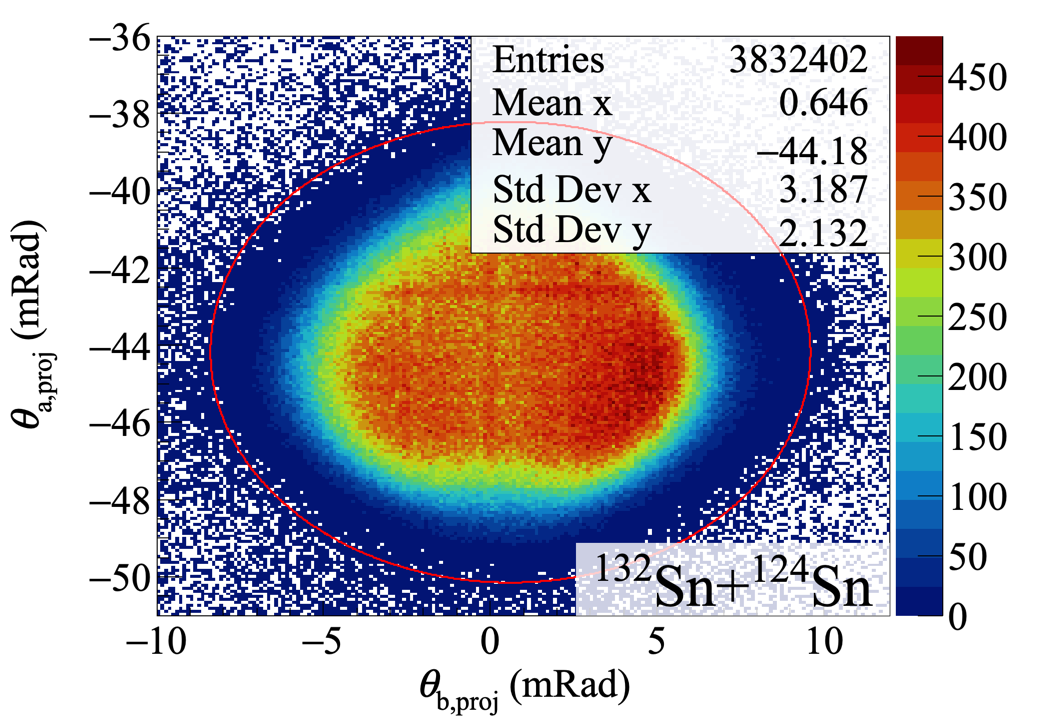
\includegraphics[width=\linewidth]{beamAngle-Sn132.png} 
        \caption{Competitors} \label{fig:mom_L_after}
    \end{subfigure}
\label{fig:mom_sc}
\end{figure}



\section{Vertex Cut}
A vertex cut on verticies originating from the target region ensure we are selecting on nuclear collisions with the target. When looking at the z-component of the verticies of all events, we can see several features which correspond to different elements within the beam line and TPC. We also note that near the expected position of the target, WHAT POSITION??, we see a large enhancement of counts which corresponds to nuclear collisions on the target. The z-component of all runs in each beam type are plotted in the range of the target region in Fig.~\ref{fig:vertexdist}. Since the target thickness was less than 1 mm, the vertex resolution achieved can be experimentally measured by fitting the vertex distribution, assuming a Gaussian distribution. The extracted vertex resolutions of each system are summarized in Table~\ref{tb:vertexresol}, with an average vertex resolution of \SI{1.2}{\centi\metre}.



\begin{table*}\centering
\ra{1.3}
\begin{tabular}{@{}rrr@{}}\toprule
\multicolumn{3}{c}{Vertex Resolution}\\
\cmidrule{1-3}
System & Mean (cm) & Sigma (cm) \\
\midrule
$\tin{132}{124}$ & -14.79  & 1.2 \\
$\tin{124}{112}$ & -14.71  & 1.1 \\
$\tin{112}{124}$ & -14.78  & 1.2 \\
$\tin{108}{112}$ & -14.75  & 1.3 \\ 
\bottomrule
\end{tabular}
\caption{Summary of measured verticies and their resolution.}
\label{tb:vertexresol}
\end{table*}



\begin{figure}[!htb]
    \centering
    \begin{subfigure}[t]{\textwidth}
        \centering
        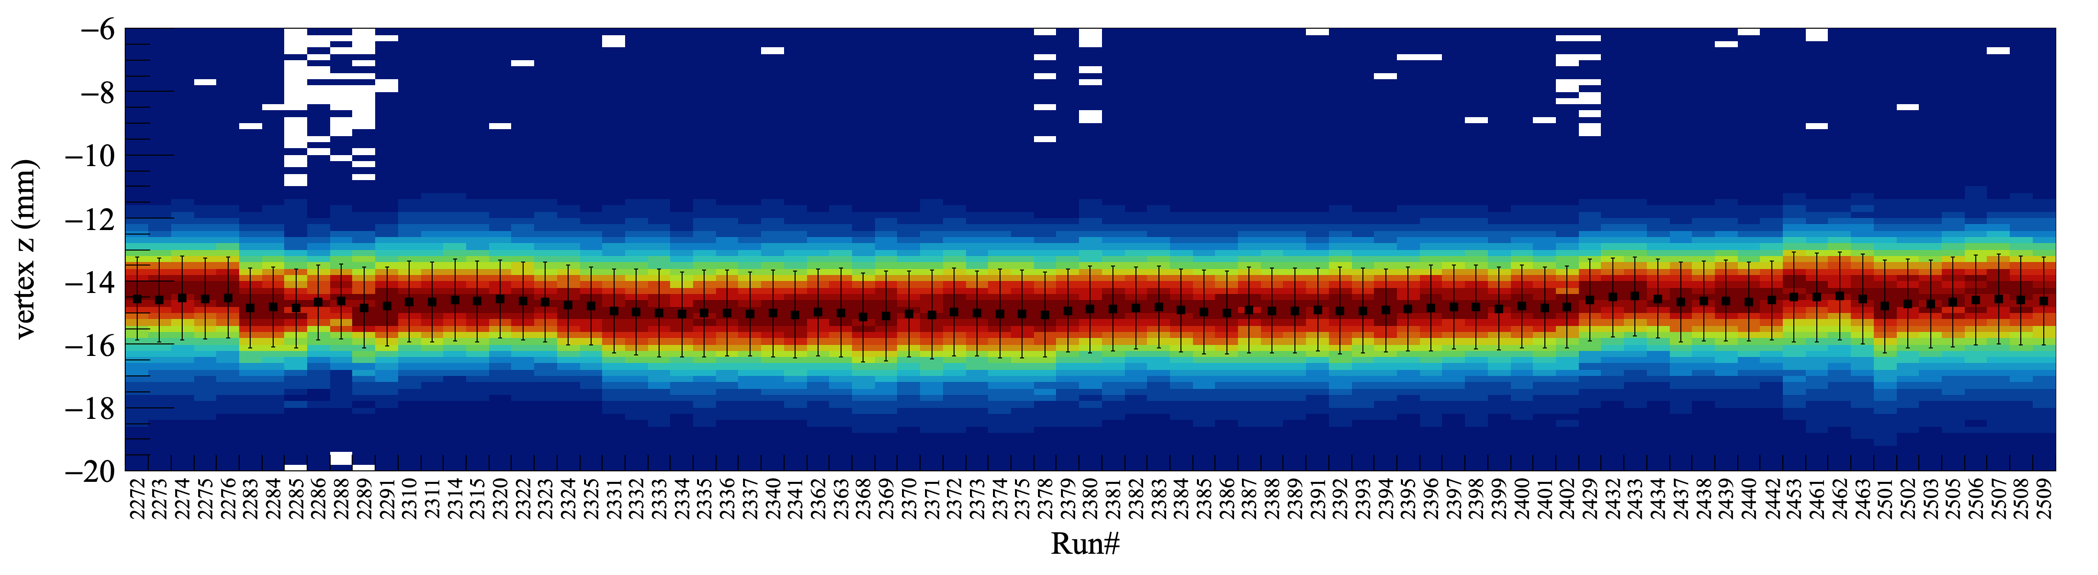
\includegraphics[width=\linewidth]{vertex-Sn108.png} 
        \caption{$\tin{108}{124}$ vertex distributon for all runs.} \label{fig:vertex108}
    \end{subfigure}
    \hfill
    \begin{subfigure}[t]{\textwidth}
        \centering
        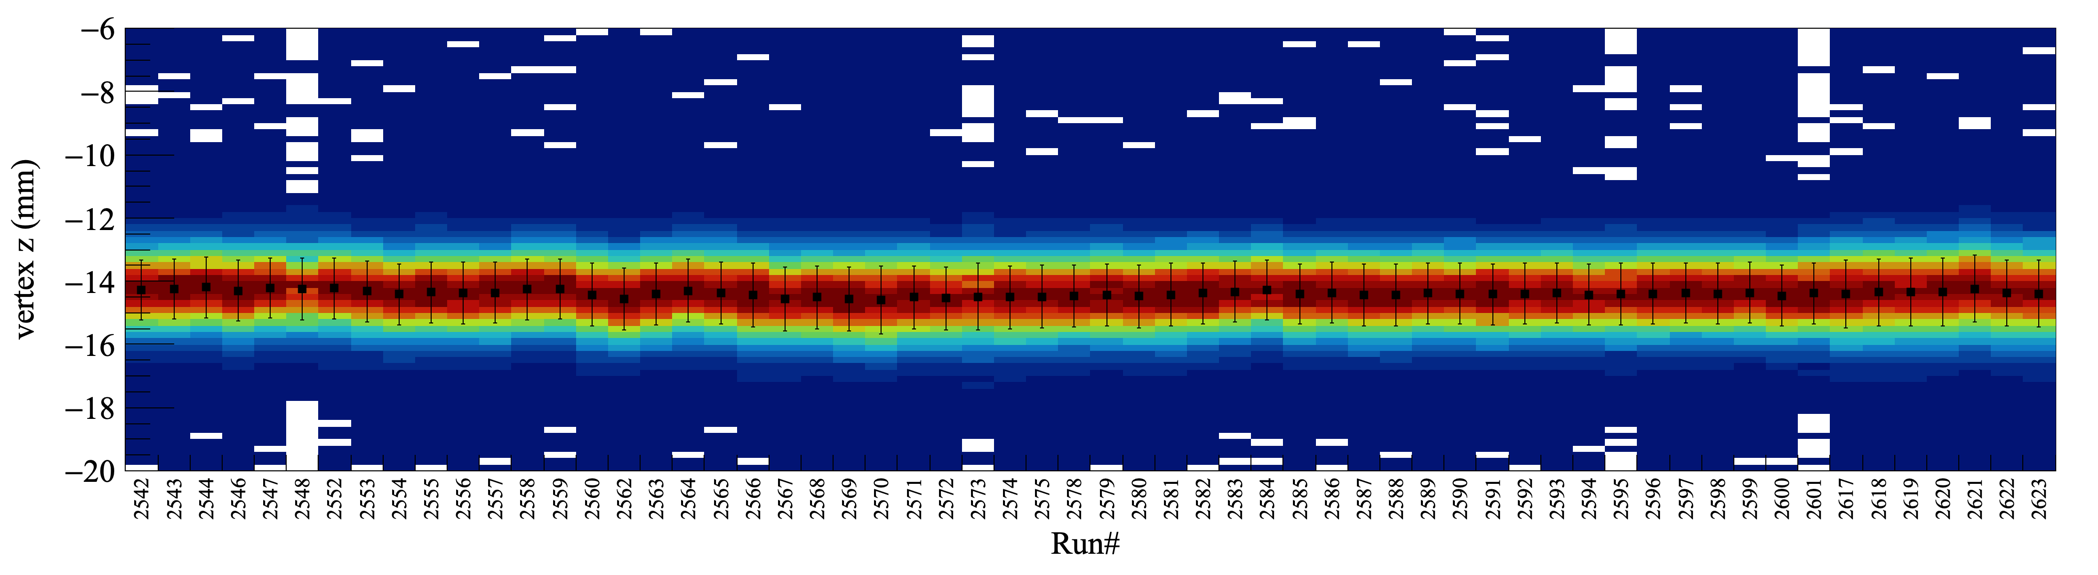
\includegraphics[width=\linewidth]{vertex-Sn112.png} 
        \caption{$\tin{112}{124}$ vertex distributon for all runs.} \label{fig:vertex112}
    \end{subfigure}
    
    \begin{subfigure}[t]{\textwidth}
        \centering
        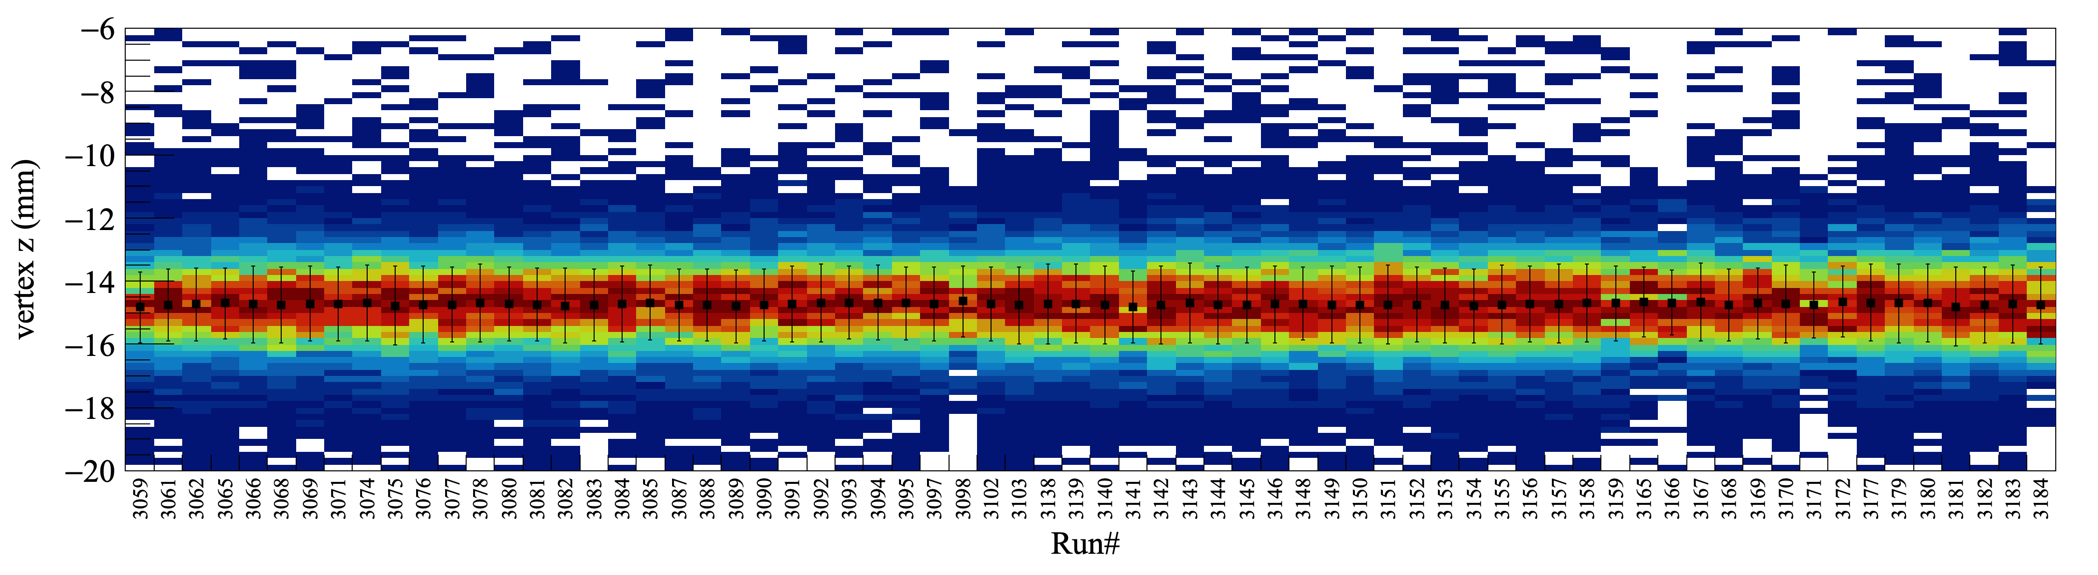
\includegraphics[width=\linewidth]{vertex-Sn124.png} 
        \caption{$\tin{124}{112}$ vertex distributon for all runs.} \label{fig:vertex124}
    \end{subfigure}
    \hfill
    \begin{subfigure}[t]{\textwidth}
        \centering
        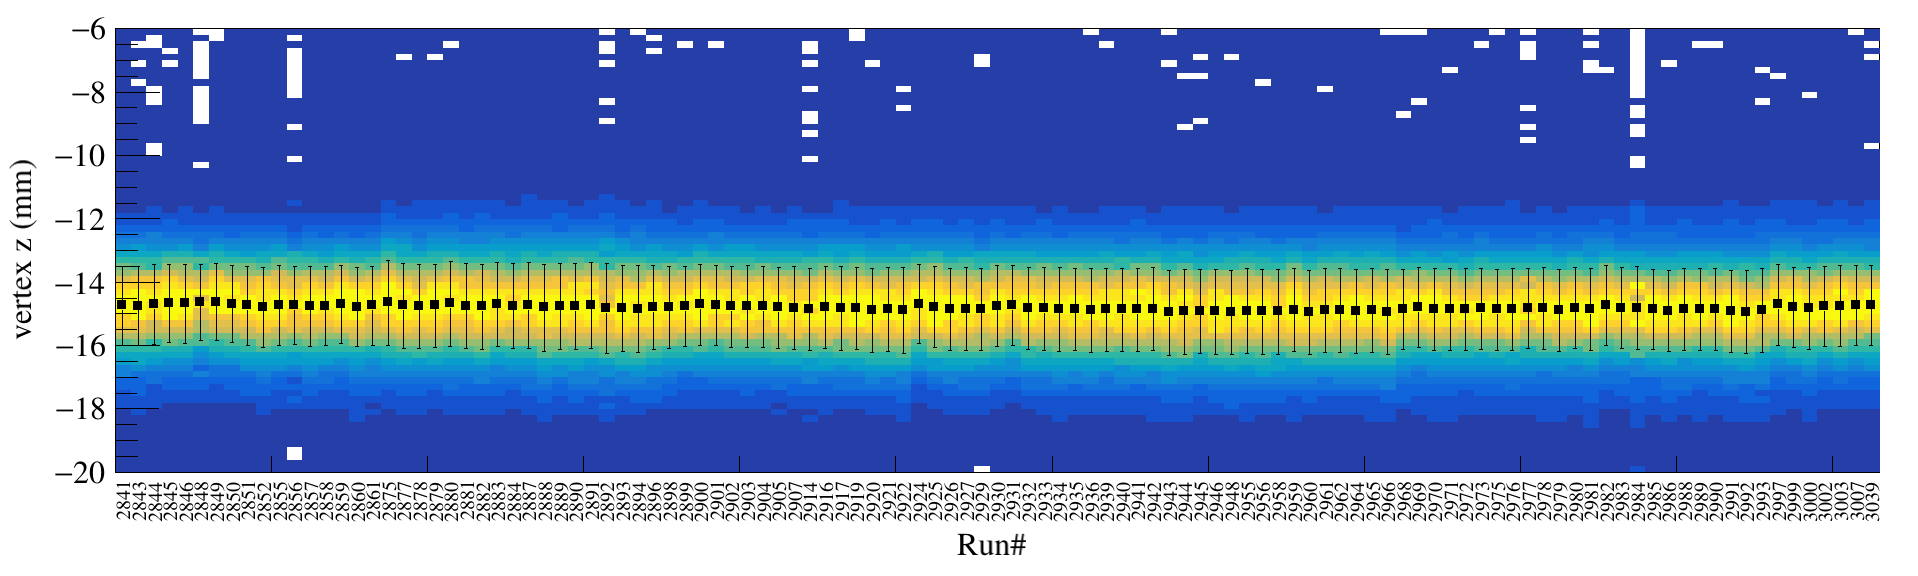
\includegraphics[width=\linewidth]{vertex-Sn132.png} 
        \caption{$\tin{132}{124}$ vertex distributon for all runs.} \label{fig:vertex132}
    \end{subfigure}
\label{fig:vertexdist}
\end{figure}


\section{Impact Parameter Selection}
The impact parameter which is defined as the distance (center-to-center), between two nuclei in a collision is a pure theoretical concept. Though experimentally there is no way in experiment to measure the impact parameter directly, several quantities have been indirectly related to the centrality of the collision CITE HERE. As discussed in Section CITE HERE, the Kyoto multiplicity array was used to experimentally trigger on central nuclear collision events. This is under the reasonable assumption that the number of charged particles in a collision grows as the impact parameter decreases. This is best described by a spectator-participant model of nuclear collisions, where a large fraction of the participating nucleons in the overlap region of the two colliding nuclei fragment into individual and clusters of nucleons. In the case where the impact parameter is zero, all the nucleons in both nuclei participate, were as larger impact parameters (peripheral collisions), less nucleons participate. 

Certainly the Kyoto array introduces a bias in our measurement of the multiplicity of all the events. At low track multiplicities, the orientation of the event starts to play a major role. Theoretically the orientation of the event (the reaction plane) is random, but due to the fact that we only measure the multiplicity on the sides of the TPC, we are preferentially triggering on events with reaction planes that emit particles in these directions. Therefore events with low track multiplicity (therefore more peripheral), that emit preferentially up and down in the TPC will not be triggered on. This becomes less of an issue as even in mid-peripheral collisions were the number of particles emitted becomes much greater than the Kyoto multiplicity selection. 

Assuming a geometric cross section $\sigma$ and the impact parameter of the collision $b$,

\begin{equation}
\sigma = \pi \cdot b^2,
\label{eq:crossSect}
\end{equation}

we can estimate the maximum impact parameter $b_{\mathrm{max}}$, by measuring the total cross section of each system. A detailed analysis on determining the cross section is given in CITE HERE. I have summarized the finding of the cross section and $b_{\mathrm{max}}$ for all the systems. Assuming $b_{\mathrm{max}}$ represents the most peripheral collisions we can define an estimate for the impact parameter $\hat{b}$, which we can define from the cumulative integral of the measured multiplicity distribution,

\begin{equation}
\hat{b} = b_{\mathrm{max}} \frac{\int_{\infty}^{M_x} f(M) dM}{\int_{\infty}^{0} f(M) dM}.
\end{equation}

 

\section{Track Quality Cuts}
%graphic showing distance to vertex, number of clusters
%number of cluster cut
%distance to vertex
In this section we will discuss the quality of the reconstructed track and will simply refer to it as the ``track quality". Certainly tracks with more clusters are of higher quality than those with few clusters. Occasionally the software will associate clusters and construct a track whose vertex does not coincide with the event vertex. This can occur for a variety of reasons. For a low momentum pion the radius of curvature is such that several rotations can occur in the event which the software can interpret as several tracks; while only one of the reconstructed track appears to originate from the event vertex. It could also happen that false tracks are created by the software from clusters which originate from several different real tracks. These are fairly obvious as they usually traverse the detector horizontally and the number of clusters is very low. In this situation the false track does not originate from anywhere near the vertex. 

To reduce the number of fake tracks, or multiple counting of tracks, a simple cut on the measurement of a track's distance to vertex can be used. The vector representing the minimum distance to vertex for each track can be calculated and its corresponding magnitude. We define the distance to vertex cut as a small sphere centered on the vertex location with a radius R. If the distance to vertex of a particular track $d_i$ < R the track is assumed to have originated from the vertex; tracks that are outside are thrown out of the analysis. 

Assuming tracks are mostly continuous in clusters, i.e. only randomly missing a few clusters, the number of clusters is directly related to the momentum resolution of a track. 


\begin{figure}[!htb]
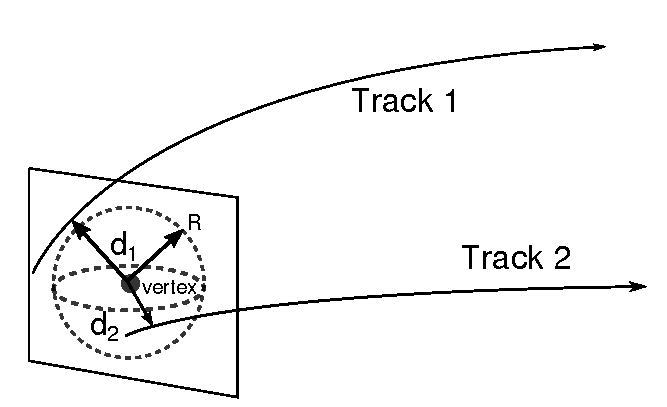
\includegraphics[width=\textwidth]{distancetovertex.pdf}
\label{fig:poca}
\caption{Distance to vertex for tracks.}
\end{figure}


\section{Angular Quality Cuts}

